\chapter{Data Privacy via Zero Knowledge Cryptography}
\section{Introduction}
In Bitcoin, the state or ledger of the system is maintained using the UTXO format, where each transaction has a list of inputs and outputs. The outputs indicate the public keys of the recipients, and the inputs refer to the outputs of previous transactions. Each UTXO has a history of transactions that can be traced back to its origin.
\begin{figure}[h!]
	\centering
	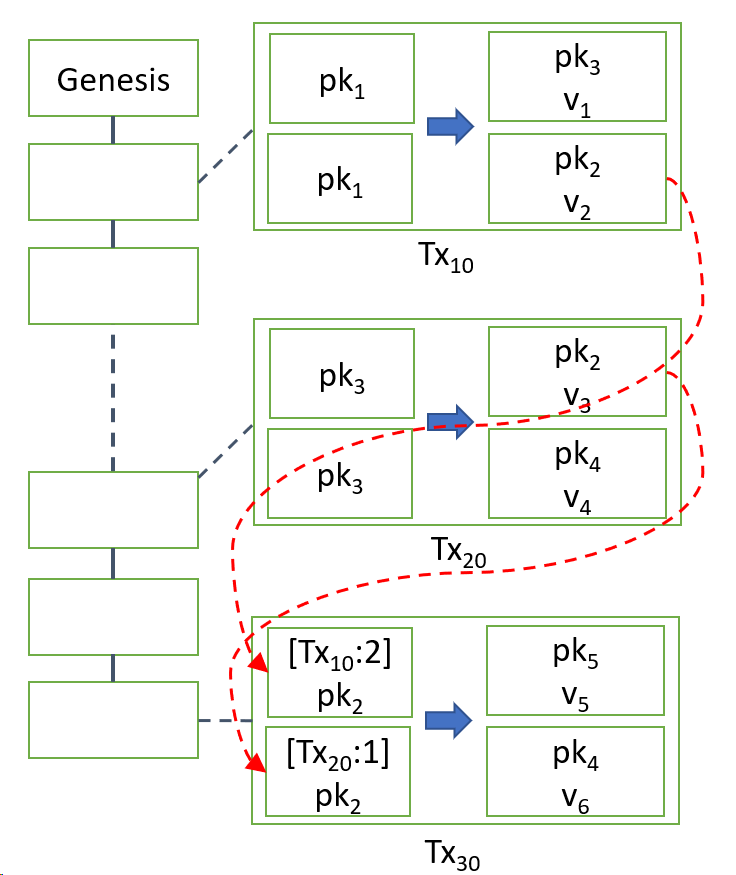
\includegraphics[width=0.25\linewidth]{Fig/19/F1}
	\caption{UTXO Transactions}
	\label{fig:L19_f1}
\end{figure}
The Bitcoin network has a feature of pseudonymity, which means that the only thing that identifies an account is the public key. A user can create many public keys to hide their identity. However, the transactions reveal some information about the connections between public keys.\\
We can use the public keys of the inputs and outputs of a transaction to create a graph that shows the links between transactions. (See Figure \ref{fig:L19_f2})
\begin{figure}[h!]
	\centering
	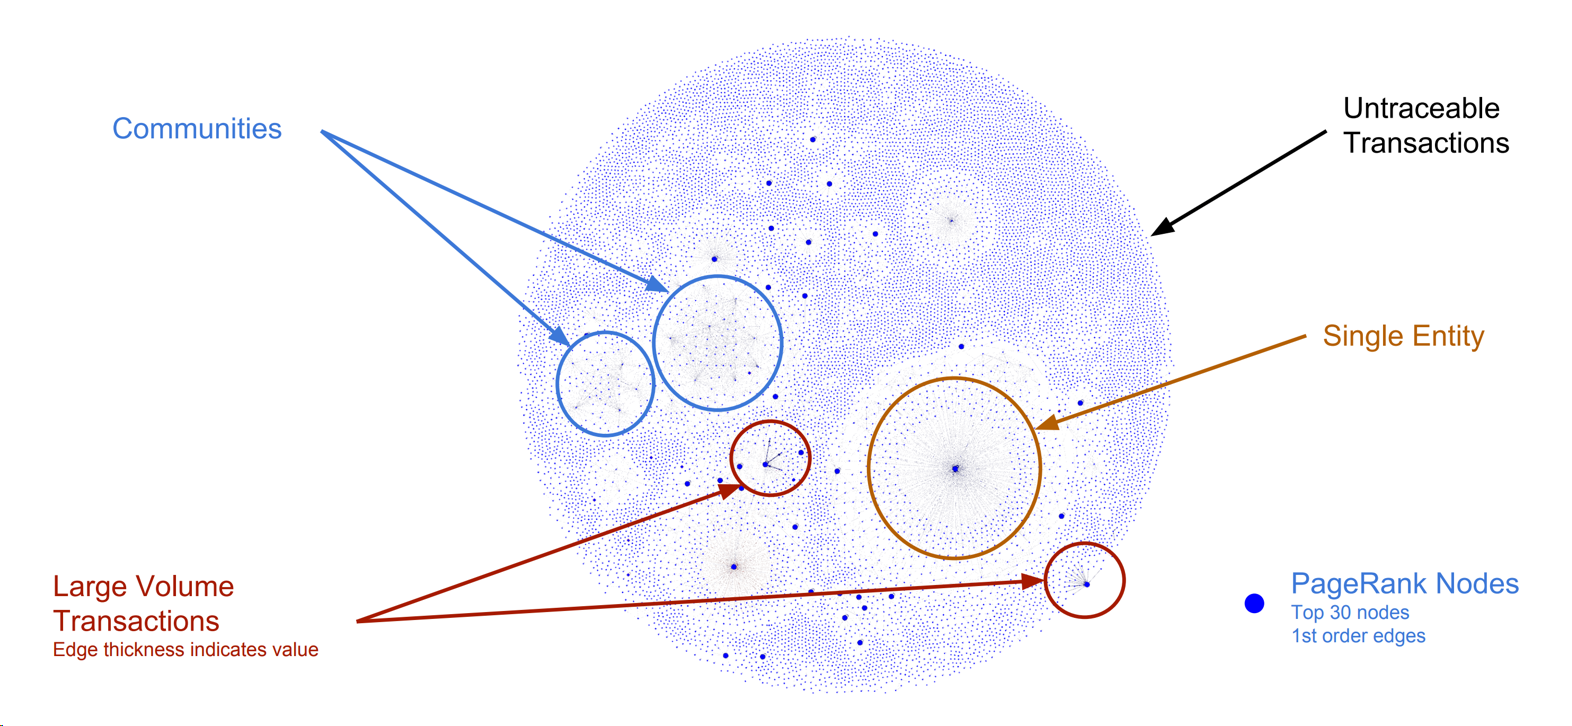
\includegraphics[width=0.8\linewidth]{Fig/19/F2}
	\caption{Typical transaction graph for a day}
	\label{fig:L19_f2}
\end{figure}

\subsection{Trusted third-party mixer}
A Trusted Third-party Mixer (also known as a "laundry service") is a service that helps users to protect their privacy on the blockchain. A mixer exchanges the coins (the public keys) of different users, so that the transaction graph cannot trace the public keys. \\\\
For example, if a user wants to make a new transaction with some outputs from previous transactions, the UTXO system needs the user to specify which outputs they will use. The mixer can exchange these outputs with other users’ outputs, so that the public keys are different.\\\\
A mixer is a centralized third-party, which means that it is controlled by a single entity. The mixer can trace or steal the coins of the users, so the users have to trust the mixer.
\ex{Coinbase}{An example of a mixer is Coinbase, which is a platform that allows users to buy, sell, and store cryptocurrency. Coinbase offers different public keys for each transaction, so that the users can hide their identity.}
\begin{figure}[h!]
	\centering
	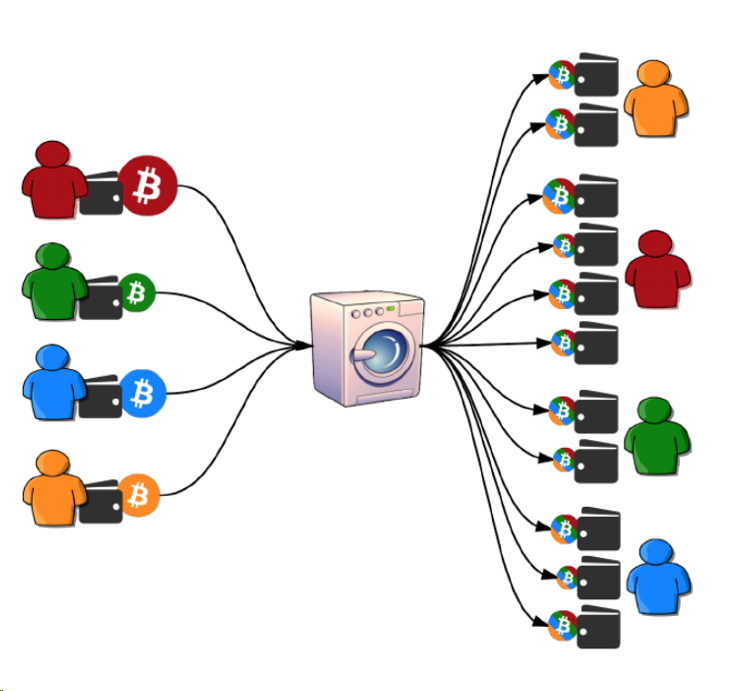
\includegraphics[width=0.3\linewidth]{Fig/19/F3}
	\caption{Trusted third-party mixer}
	\label{fig:L19_f3}
\end{figure}
\section{Zero-knowledge proof}
To achieve a decentralized privacy service that is compatible with the UTXO format, we can eliminate the need for a trusted party in the laundry system. We can do this by using a special UTXO transaction that has an input and an output. Instead of linking the input to a specific previous output, we attach a proof to the input. The proof is valid if it can show that the sender owns the input coin and has not spent it. However, the proof does not reveal which output the input coin comes from.\\
The property of not revealing connections between inputs and outputs can be achieved by
zero-knowledge proofs.
\subsection{Zerocoin}
Zerocoin is a protocol that enhances the privacy of Bitcoin transactions. Zerocoin allows users to convert their bitcoins into zerocoins, which are anonymous tokens that can be redeemed for bitcoins later. Zerocoins are stored in a separate ledger on the blockchain, and their origin and destination are hidden by using \textbf{zero-knowledge proofs}.\\\\
\begin{figure}[h!]
	\centering
	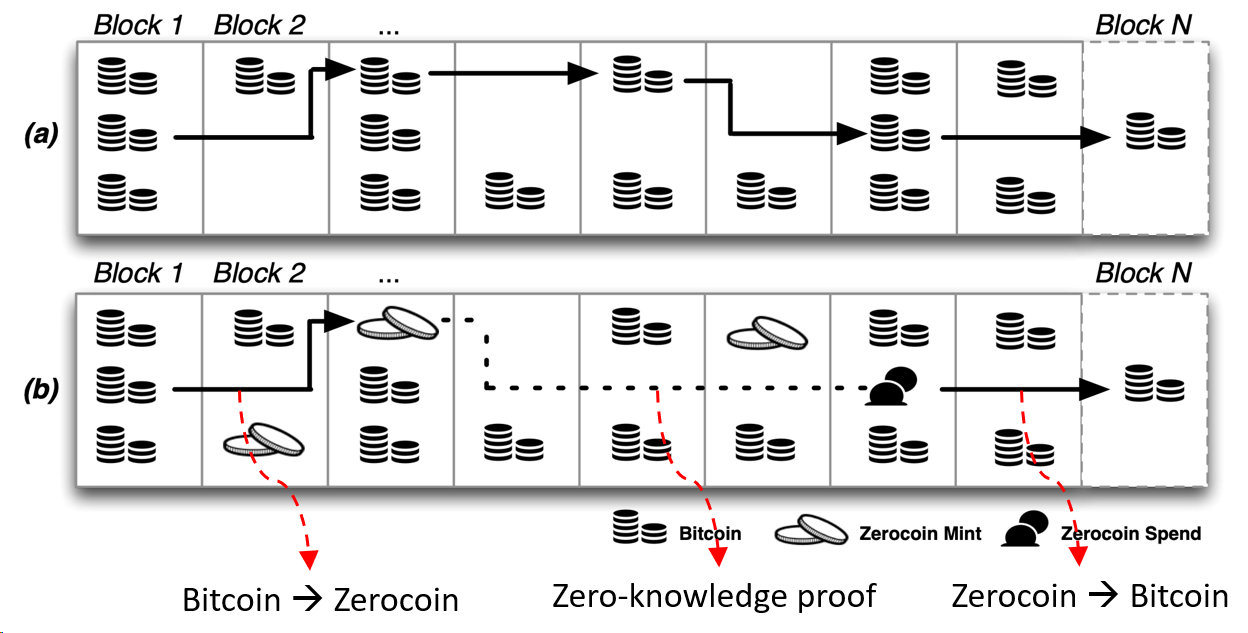
\includegraphics[width=0.6\linewidth]{Fig/19/F4}
	\caption{Zerocoin}
	\label{fig:L19_f4}
\end{figure}
Zero-knowledge proofs are cryptographic techniques that allow users to prove that they own some zerocoins without revealing which ones. Zerocoin is a decentralized laundry system, which means that it does not rely on any trusted third-party to mix the coins. (See Figure \ref{fig:L19_f4})\\
However, Zerocoin has some drawbacks, such as large overhead, limited functionality, and vulnerability to attacks.

\subsection{Zcash}
One of the most efficient cryptographic methods to create zero-knowledge proofs is zk-SNARK, which stands for "zero-knowledge, succinct and non-interactive arguments of knowledge". A zk-SNARK proof is short and easy to verify.\\\\
Zcash is a cryptocurrency that enhances the privacy of Bitcoin transactions by using the UTXO framework and the zk-SNARK cryptographic tool. Zcash introduces new types of transactions that hide the origin, destination, and amount of the payment. These transactions also allow the coins to be split and merged.\\\\
Zcash uses zk-SNARK to create efficient proofs that replace the traditional links between inputs and outputs. The proof shows that : 
\begin{itemize}
	\item the sender has the secret keys that match some of the public keys of previous outputs (the set of outputs is hidden)
	\item the sender does not spend more than the total amount of these outputs.
\end{itemize}
This helps to conceal both the identity and the value of the coins transferred.
\begin{figure}[h!]
	\centering
	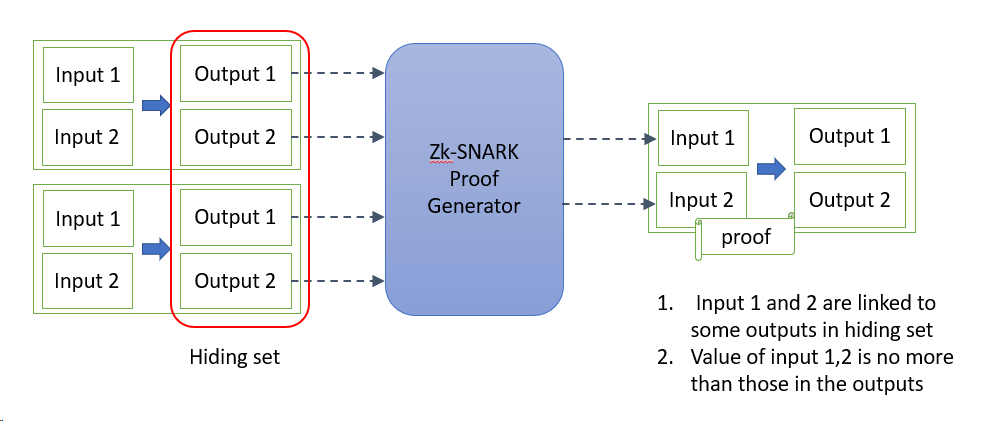
\includegraphics[width=0.6\linewidth]{Fig/19/F5}
	\caption{Zcash}
	\label{fig:L19_f5}
\end{figure}

\section{Zero-knowledge Model}
\subsection{Language and NP}
\dfn{Language}{A language L is a set of statements such that
	\begin{align*}
		L(x) = 1 \qquad \text{if} \quad x \in L
\end{align*}}
Language is a way of defining a set of statements that have a certain property. For example, the language of composite numbers is the set of statements that say that a number is composite, which means that it has more than two factors.\\
\dfn{NP}{We define NP to be the class of languages $L$ that have a polynomial time Verifier $V$, such that
	\begin{align*}
		L(x) = 1 \Leftrightarrow \exists w, \quad \text{s.t.} \quad V (x,w) = 1
\end{align*}}
NP is a way of defining a class of languages that have a certain property. For example, the class of languages that can be verified in polynomial time by a verifier. A verifier is an algorithm that takes two inputs: a statement and a witness. A witness is an additional piece of information that helps to prove the statement.
\ex{NP}{x is an integer, L is testing for composite. We can find a witness
	here to be the prime factorization of x, and the verifier can testify whether the product of w
	equals to x in polynomial time.}

\subsection{Prover and Zero-knowledge}
Prover and Zero-knowledge are two roles that are involved in a zero-knowledge proof. \\
For example, if the statement is that a number x is composite, then the Prover is the one who knows the factorization of x, and the Verifier is the one who wants to check if the statement is true.The Prover can send x and its factors w to the Verifier, and claim that x is composite. The Verifier can then ask the Prover to prove it by using some mathematical technique that does not reveal w. This way, the Verifier can be convinced that x is composite, but cannot learn anything about w.
\begin{figure}[h!]
	\centering
	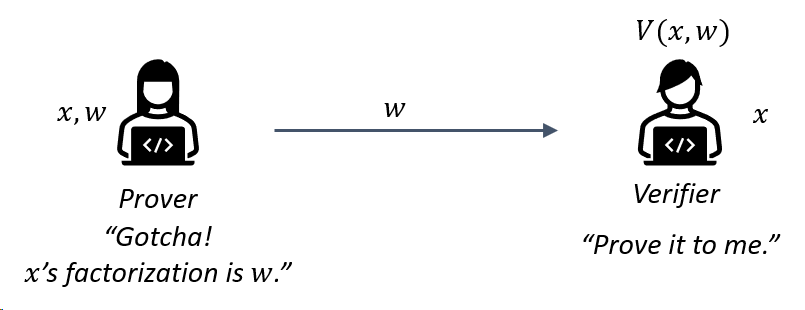
\includegraphics[width=0.5\linewidth]{Fig/19/F6}
	\caption{Prover and Verifier}
	\label{fig:L19_f6}
\end{figure}\\
A zero-knowledge proof system has three security requirements:
\begin{itemize}
	\item \textbf{Completeness}: This means that if the statement is true and the prover knows a valid witness, then the prover can always persuade the verifier to accept the proof.
	\item \textbf{Soundness}: This means that if the statement is false ($x \notin L$), then the verifier cannot be fooled by any prover to accept the proof.
	\item \textbf{Zero-knowledge}: This means that the proof does not reveal any information about the witness or any other secret information to the verifier.
\end{itemize}
Imagine that you have a number $x$ and you want to prove that you know another number $w$ that satisfies the equation $g^w = x$, where g is a special number that can generate a group of numbers with a prime size $q$. To achieve zero-knowledge, the verifier only has access to $x$ and should learn nothing about $w$ during the verification process.
The proof is done by following these steps:
\begin{enumerate}
	\item The prover picks a random $v \in \mathbb{Z}^*_q$, and sends the verifier $t = g^v$.
	\item The verifier chooses a random number $c \in \mathbb{Z}^*_q$, and sends it back to the prover.
	\item The prover computes $r = v - cw$ and returns $r$ to the verifier.
	\item Finally, the verifier checks if $t = g^r \, x^c$
\end{enumerate}
\begin{figure}[h!]
	\centering
	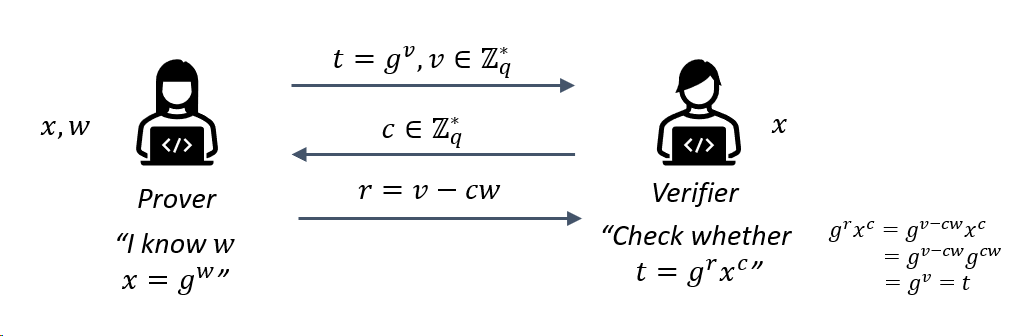
\includegraphics[width=0.7\linewidth]{Fig/19/F7}
	\caption{Zero-knowledge proof}
	\label{fig:L19_f7}
\end{figure}
As we can see, the proof and verification process do not reveal anything about w, because it is hidden by random numbers. This is why it is called "zero knowledge". The amazing thing is that every problem in NP has a zero knowledge proof.

\subsection{Efficiency}
The efficiency of the cryptographic tools (e.g., how much time they need to create the proof or check the proof, how big the proof is) is important for practical use. We use T to represent the time it takes to run V(x,w), which is the basic complexity of verification. We look at four measures of complexity of zero knowledge proof systems :
\begin{itemize}
	\item \textbf{Prover complexity} : Provers who are efficient can make proofs in an expected time of $O(T \log T)$. This is only slightly more than the basic complexity.
	\item \textbf{Verification complexity and proof size.} : A good feature of these proof systems is that they are succinct, which means that the proof size is small and can be checked quickly. The proof size can be constant or logarithmic compared to the statement size. The proof can be verified in an expected time of O(1) or O(log T), which means that it does not depend on the statement size. However, the verification is still not very efficient for practical use (for example, in Zcash), because the constants are large.
	\item \textbf{Interactivity of verification} : Many zero knowledge protocols require interaction between the prover and the verifier. However, noninteractive proofs are more suitable for blockchain applications. There is a general technique to make interactive protocols noninteractive while keeping their security properties (this is called the Fiat-Shamir heuristic), but it works under ideal conditions (including needing a special model called random oracle) and it is not very practical. Therefore, we are interested in finding more specific approaches for noninteractive proofs.
	\item \textbf{Setup assumptions} : Some zero knowledge protocols need a "trusted setup", for example, zk-SNARKs. This means that a trusted party has to compute the parameters that are needed to make and check the proofs. If this party is not honest, the protocol could be broken and the money could be created out of thin air. To avoid this, some protocols like zk-STARKs (Zero-Knowledge Scalable Transparent ARguments of Knowledge) use public randomness instead of trusted setup to create systems that can be verified without trusting anyone. These systems are based on advanced cryptography and are being developed into practical libraries by researchers.
\end{itemize}

\section{From Zero Knowledge Proof Systems to Zcash}
We create new data structures and ways of addressing on top of Bitcoin’s design to enable anonymity in Bitcoin using zero knowledge proof systems.
\begin{itemize}
	\item \textbf{Address} :  Like Bitcoin, Zcash has two kinds of addresses: public key address $addr_{pk}$ and secret key address $addr_{sk}$.
	\item We define a coin c, which has the same role as a transaction output of Bitcoin, with the following attributes:
	\begin{itemize}
		\item Coin commitment $cmt(c)$
		\item Coin value $v(c)$
		\item Coin serial number $sn(c)$
		\item Coin address $addr_{pk}(c)$
	\end{itemize}
	The coin commitment is a way of hiding the data inside the coin by using a special function that produces a unique output for each input. The serial number is a way of identifying the coin by using another function that produces a random-looking output for each input. Both functions are based on a mathematical operation called SHA256 compression, which is also used to create the addresses and the coin attributes.
	
	\item \textbf{Pour transaction structure} : A pour transaction is a type of transaction that has two inputs and two outputs. Unlike Bitcoin transactions, the pour transaction only shows the serial numbers of the coins that are used as inputs, but it hides everything else, such as how much money the coins are worth, or who owns them.\\\\
	All the	publicly visible information of the transaction can be denoted as : 
	\begin{align*}
		tx := (rt; sn_1^{old}; sn_2^{old}; cmt_1^{new}; cmt_2^{new}; v_{pub}; \text{info}; \text{proof})
	\end{align*}
	which $rt$ is the Merkle root; inputs, which are the serial numbers of the old coins; outputs, which are the commitments of the new coins; $v_{pub}$, which is the part of the input value that can be optionally revealed to the public; info, which is a transaction string that can be optionally added; and proof, which is used to show that the old coins belong to the sender and that the transaction is valid. The pour transaction allows both splitting and merging of the coins by using two inputs and outputs. This means that multiple coins can be split or merged by using multiple pour transactions. We will explain these properties in more detail below.
\end{itemize}
\begin{figure}[h!]
	\centering
	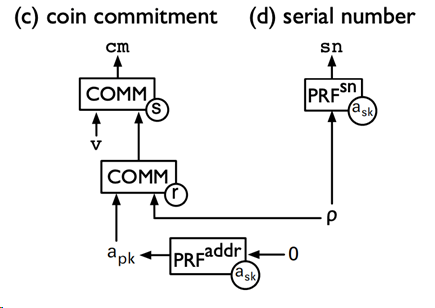
\includegraphics[width=0.3\linewidth]{Fig/19/F8}
	\caption{Data structure}
	\label{fig:L19_f8}
\end{figure}

\section{Zcash Framework}
Our goal is to design a pour transaction that hides the details of the coins (especially the public keys) that are involved in creating two new coins from two old coins. This is the transaction linkage problem that Bitcoin’s UTXO state management system has to deal with.

\subsection{First Attempt: use commitment}
First We try to construct the transaction using only the coin commitments, i.e. a pour transaction has \\
$(cmt_1^{old} , cmt_2^{old}, cmt_1^{new}, cmt_2^{new} , \text{proof})$ as its components.\\\\
The problem formulation can be expressed as an NP statement, abstracting away the details of how the zero knowledge proof is generated. The statement includes:
\begin{itemize}
	\item $ x = (cmt_1^{old} , cmt_2^{old}, cmt_1^{new}, cmt_2^{new}) $
	\item $L(x)$ is an indicator of whether $x$ is a valid pour transaction. $L(x) = 1$ if $x$ is a valid pour transaction.
	\item $w = \left(c_1^{old}, c_2^{old}, c_1^{new}, c_2^{new}, addr_{sk}(c_1^{old}), addr_{sk}(c_2^{old})\right)$
\end{itemize}
Given $x$ and $w$, a verifier $V(x,w) = 1$ if the following conditions are true:
\begin{itemize}
	\item The commitments of four coins are correct
	\item $v(c_1^{old} )+v(c_2^{old} ) \ge v(c_1^{new} )+v(c_2^{new})$
	\item $addr_{sk}$ of two old coins matches $addr_{pk}$ 
\end{itemize}
It is easy to see that $L(x) = 1 \Leftrightarrow V(x,w) = 1$.\\\\
We use algebraic circuits to represent these statements and generate the proof by \textbf{circuit satisfiability}. The proof is an encrypted pair $\pi = [g^H, g^Z]$, where $H$ and $Z$ are polynomials that are calculated during the proving phase, and there is a verification key $vk = g^T$. We saw in the discrete logarithm example above that the proving process did not expose the witness information because it is hard to invert the logarithm. You can read more about an example construction in this \href{https://medium.com/@VitalikButerin/quadratic-arithmetic-programs-from-zero-to-hero-f6d558cea649}{post}.\\\\
Now anyone in the blockchain who has access to $w$ can produce the proof without revealing any information related to $w$, and anyone who has access to $x$ can check the validity of the transaction. But this method has a weakness that the commitment can still be traced.
\begin{figure}[h!]
	\centering
	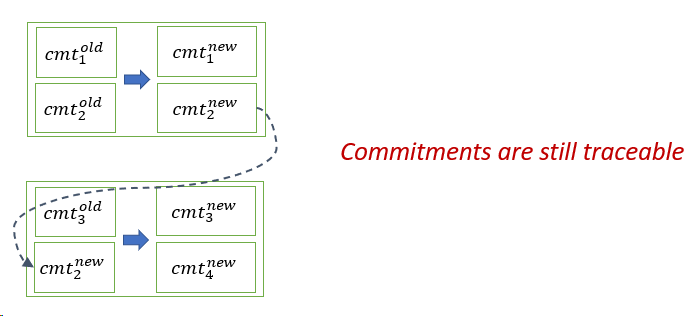
\includegraphics[width=0.6\linewidth]{Fig/19/F9}
	\caption{First attempt: Commitment}
	\label{fig:L19_f9}
\end{figure}

\subsection{Second Attempt: two commitments}
A possible improvement on the previous approach is to use two kinds of commitments:
\begin{enumerate}
	\item a regular commitment $cmt$
	\item a unique serial number $sn$ (created by a pseudo-random generator)
\end{enumerate}
In a transaction, we use serial numbers to represent the old coins and commitments to represent the new coins, i.e., the transaction contains $(rt; sn_1^{old}, sn_2^{old}, cmt_1^{new}, cmt_2^{new}, \text{proof})$, where $rt$ indicates the Merkle-tree root of the commitments of the outputs in the ledger. The witness remains the same,
\begin{align*}
	w = \left(c_1^{old}, c_2^{old}, c_1^{new}, c_2^{new}, addr_{sk}(c_1^{old}), addr_{sk}(c_2^{old})\right)
\end{align*}
And again $L(x) = 1$ if and only if $V(x,w) = 1$, $V(x,w) = 1$ if the following conditions hold:\\
For $i \in \{1, 2\}$:
\begin{itemize}
	\item The commitments $cmt_i$ of $c_i^{new}$ appear on the ledger, verified using the Merkle-tree root $rt$, i.e.
	\begin{align*}
		cmt(c_1^{new}) \in rt \wedge cmt(c_2^{new}) \wedge rt
	\end{align*}
	\item The address secret key $addr_{sk}^{old},_i$ matches the address public key of $c_i^{old}$.
	\item $\left(sn(c_1^{old}), sn(c_2^{old}), cmt(c_1^{new}), cmt(c_2^{new})\right) = \left(sn_1^{old}, sn_2^{old}, cmt_1^{new}, cmt_2^{new}\right)$
	\item $v(c_1^{old} )+v(c_2^{old} ) \ge v(c_1^{new} )+v(c_2^{new})$
\end{itemize}
\begin{figure}[h!]
	\centering
	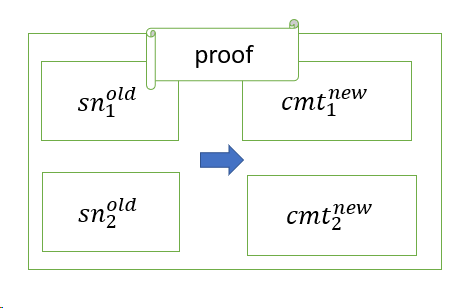
\includegraphics[width=0.25\linewidth]{Fig/19/F10}
	\caption{Second Attempt: two commitments}
	\label{fig:L19_f10}
\end{figure}
This formulation is similar to the previous one, in that those who possess $w$ can create the proof and those who possess $x$ can verify the validity. However, unlike the previous method, there is no direct link between the old coins and the new coins since they use different kinds of commitments. The only issue is that without the link, how can we tell which previous output is being spent? To address this issue, we keep track of all serial numbers that appear in previous transactions as a nullifier set and perform an extra check to see if the input serial number is already in the nullifier set.
\begin{figure}[h!]
	\centering
	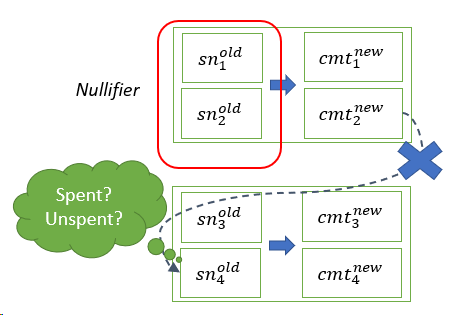
\includegraphics[width=0.5\linewidth]{Fig/19/F11}
	\caption{Check Unspent Coins}
	\label{fig:L19_f11}
\end{figure}

\section{Zcash Protocol: Putting it all together}
Zcash modifies Bitcoin by introducing pour transactions. Unlike a normal UTXO transaction, the pour transaction uses commitments and serial numbers instead of inputs and outputs to hide the connection between the old and new coins.
\subsection{Create a pour transaction}
The complete structure of a pour transaction, as we defined earlier, consists of 
\begin{align*}
	(rt; sn_1^{old}; sn_2^{old}; cmt_1^{new}; cmt_2^{new}; v_{pub}; \text{info}; \text{proof})
\end{align*}
To make a pour transaction, the sender needs the following information:
\begin{itemize}
	\item Old coins $c_1^{old} \,\, , \,\, c_2^{old}$
	\item Secret keys of old coins $addr_{sk}(c_1^{old}) \,\, , \,\, addr_{sk}(c_2^{old})$
	\item New values $v_1^{new} \,\, , \,\, v_2^{new}$
	\item Public value $v_{pub}$ s.t. $v_1^{old} + v_2^{old} \ge v_1^{new} + v_2^{new} + v_{pub}$
	\item New addresses $addr_{sk}(c_1^{new}) \,\, , \,\, addr_{sk}(c_2^{new})$
\end{itemize}
\begin{figure}[h!]
	\centering
	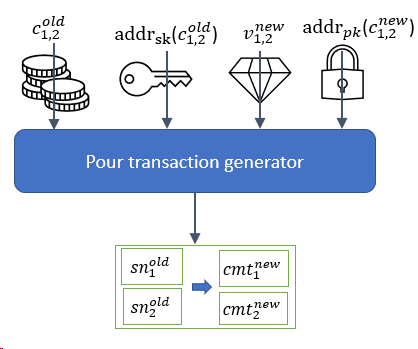
\includegraphics[width=0.4\linewidth]{Fig/19/F12}
	\caption{Generate a pour transaction}
	\label{fig:L19_f12}
\end{figure}
A real system can use a transaction generator to create a pour transaction and the new coins for the sender, given the necessary information. The sender then sends the new coins to the recipients off chain and the transaction is broadcasted on chain.

\subsection{Generate a zk-SNARK proof}
zk-SNARK is a cryptographic method that allows zero knowledge, succinct and non-interactive verification. It means that a prover who has a witness for an NP-statement can generate a short proof that anyone can verify without revealing the witness. The NP-statements in Zcash are usually statements of satisfiability, such as "the input matches this specific value for this specific hash function".\\\\
There are three polynomial time algorithms involved in the proving process, which are part of a library.
\begin{itemize}
	\item \textbf{KeyGen} : KeyGen is the trusted setup that creates the proving and verifying keys, pk and vk, once for all.
	\item \textbf{Prove} : The function Prove takes $pk$, the witness $w$ and the public input $x$ and produces a short proof $\pi= Prove(pk, w, x)$.
	\item \textbf{Verify} : The function Verify takes $vk$, the public input $x$ and the proof $\pi$ and outputs a Boolean value $Verify(vk, x, \pi)$.
\end{itemize} 
\begin{figure}[h!]
	\centering
	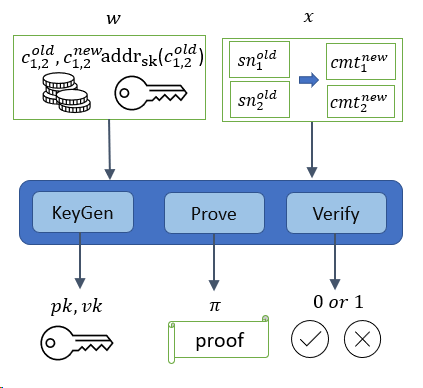
\includegraphics[width=0.4\linewidth]{Fig/19/F13}
	\caption{Generate a zk-SNARK proof}
	\label{fig:L19_f13}
\end{figure}

\subsection{Incentives in Zcash}
Zcash is a privacy-enhanced version of Bitcoin that uses the same basic protocol with an added feature of hiding transaction details. The incentives in Zcash are the same as in the Bitcoin protocol, which include both mining rewards and transaction fees. Since the zk proof verification process is fast, the verification time does not increase much (especially compared to the slow mining rate in Bitcoin).

\section{Privacy}
Privacy refers to how well the transactions hide the details of the sender, receiver, and amount. Programmability refers to how flexible the transactions support smart contracts, which are self-executing agreements with complex rules and logic.
\begin{figure}[h!]
	\centering
	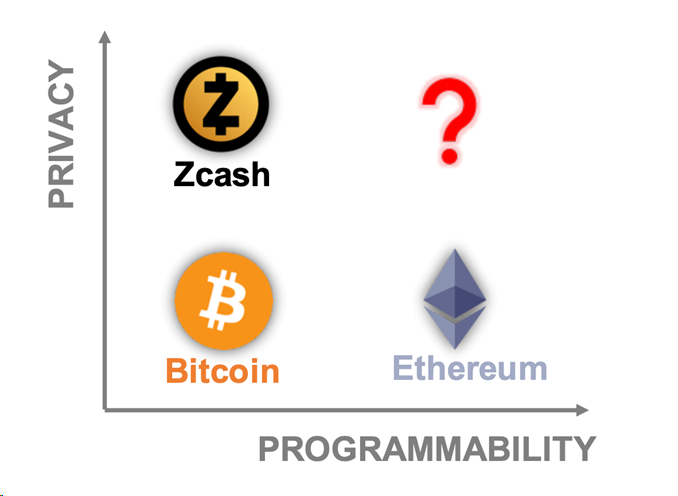
\includegraphics[width=0.4\linewidth]{Fig/19/F14}
	\caption{Cryptocurrencies in term of privacy and Programmability}
	\label{fig:L19_f14}
\end{figure}\\
Figure \ref{fig:L19_f14} shows that Zcash has high privacy and low programmability, Bitcoin has low privacy and low programmability, and Ethereum has low privacy and high programmability.
